% -----------------------------------------------
% Template for ISMIR Papers
% 2025 version, based on previous ISMIR templates

% Requirements :
% * 6+n page length maximum
% * 10MB maximum file size
% * Copyright note must appear in the bottom left corner of first page
% * Clearer statement about citing own work in anonymized submission
% (see conference website for additional details)
% -----------------------------------------------

\documentclass{article}
\usepackage[T1]{fontenc}
\usepackage[utf8]{inputenc}
\usepackage[submission]{ismir} % Remove the "submission" option for camera-ready version
\usepackage{amsmath,cite,url}
\usepackage{graphicx}
\usepackage{listings}
\usepackage{color}

\definecolor{dkgreen}{rgb}{0,0.6,0}
\definecolor{gray}{rgb}{0.5,0.5,0.5}
\definecolor{mauve}{rgb}{0.58,0,0.82}

\lstset{frame=tb,
  language=Python,
  aboveskip=3mm,
  belowskip=3mm,
  showstringspaces=false,
  columns=flexible,
  basicstyle={\small\ttfamily},
  numbers=none,
  numberstyle=\tiny\color{gray},
  keywordstyle=\color{blue},
  commentstyle=\color{dkgreen},
  stringstyle=\color{mauve},
  breaklines=true,
  breakatwhitespace=true,
  tabsize=3
}

% Title. Please use IEEE-compliant title case when specifying the title here,
% as it has implications for the copyright notice
% ------
\title{Progress Report and revamped timeline for Sound Visualizer}

% Note: Please do NOT use \thanks or a \footnote in any of the author markup

% Single address
% To use with only one author or several with the same address
% ---------------

\author{
  Ethan Huang\\
  \texttt{ethanhuang@uvic.ca}
  \and
  Brian Pham\\
  \texttt{npham49@uvic.ca}
  \and
  Benjamin Say\\
  \texttt{benbsay@gmail.com}
}
%%-------------- i couldn't get normal author thing in template
%% ------------ to work so idk if this is how it should look for
%% ------------- multiple author works, will have to double check

%\oneauthor
%  {Anonymous Authors}
%  {Anonymous Affiliations\\\texttt{anonymous@ismir.net}}
% Two addresses
% --------------
%\twoauthors
%   {First author} {School \\ Department}
%   {Second author} {Company \\ Address}

% Three addresses
% --------------
%\threeauthors
%    {Ethan Huang} {Affiliation 1 \\ \texttt{author1@ismir.edu}}
%   {Brian Pham} {Affiliation 2 \\ \texttt{author2@ismir.edu}}
%   {Benjamin Say} {Affiliation 3 \\ \texttt{author3@ismir.edu}}

% Four or more addresses
% OR alternative format for large number of co-authors
% ------------
% \multauthor
%   {First author$^1$ \hspace{1cm} Second author$^1$ \hspace{1cm} Third author$^2$}
%   {{\bf Fourth author$^3$ \hspace{1cm} Fifth author$^2$ \hspace{1cm} Sixth author$^1$}\\
%   $^1$ Department of Computer Science, University, Country\\
%   $^2$ International Laboratories, City, Country\\
%   $^3$ Company, Address\\
%   {\tt\small CorrespondenceAuthor@ismir.edu, PossibleOtherAuthor@ismir.edu}
%   }

% For the author list in the Creative Common license, please enter author names.
% Please abbreviate the first names of authors and add 'and' between the second to last and last authors.
\def\authorname{E. Huang, B. Pham, and B. Say}

% Optional: To use hyperref, uncomment the following.
% \usepackage[bookmarks=false,pdfauthor={\authorname},pdfsubject={\pdfsubject},hidelinks]{hyperref}
% Mind the bookmarks=false option; bookmarks are incompatible with ismir.sty.

\sloppy % please retain sloppy command for improved formatting

\begin{document}

\maketitle

\begin{abstract}
%The abstract should be placed at the top left column and should contain about 150--200 words.sdkfljasd
This project aims to recreate popular visualization features similar to those built into classic multimedia programs. We seek to implement the visualization of different frequencies in music through the use of Python and Pygame.
\end{abstract}

\section{Introduction}\label{sec:introduction}
%This template includes all the information about formatting manuscripts for the ISMIR \conferenceyear\ Conference. Please follow these guidelines to give the final proceedings a uniform look. Most of the required formatting is achieved automatically by using the supplied style file (\LaTeX) or template (Word). If you have any questions, please contact the Program Committee (\texttt{ismir\conferenceyear-papers@ismir.net}). This template can be downloaded from the ISMIR \conferenceyear\ website (\texttt{https://ismir\conferenceyear.ismir.net}).

\subsection{Background}
During the 2000s, multimedia software such as iTunes and Windows Media Player came equipped with a functionality called visualization. Behind the scenes, the visualizer takes different frequencies over the track and generates detailed geometric sequences. Our project goal is to recreate this functionality with Python. 

\subsection{High-level summary}
On a high level, sounds are combinations of different frequencies; through the usage of Pygame's rendering capabilities, each frequency can be mapped into different objects in a 2-dimensional space, allowing for visualization. Pygame's rendering engine allows for different visual manipulation techniques such as resizing, colour switch, and masking, which can handle complex frequency changes and combinations. 

\subsection{Related works}
%maybe need background/related work? Done!

\begin{itemize}
    \item Music Visualization using frequencies \cite{djfun}
    \item Music Visualization GUI \cite{avirzayev}
    
\end{itemize}

\section{Graphical Output}

\subsection{Overview}
Graphical Output is generated using a combination of Cartesian Coordinate conversion and Pygame rendering methods. By taking in the frequencies available and their magnitude at each frame, the code generate the appropriate visualization within that frame.

\subsection{Input parameters and assumptions}
The code takes the same input as following: screen, xf, yf, color; each signifying the following:
\begin{itemize}
    \item screen: The Pygame surface to render on to, by passing a surface between each rendering functions, renders would display consistently on 1 surface \cite{kinsley}
    \item xf: The available frequencies in that frame
    \item yf: The magnitude of the available frequencies in that frame
    \item color: Color of the visualization, this defaults to BLUE
\end{itemize}

The available colors are declared as items in a Dictionary to be looked up within visualization code, all that needs to be passed to the functions are the plain capitalized English word representing the color. The following colors are available with their respective RGB values: "BLUE" (100, 100, 255), "RED": (255, 50, 50), "GREEN": (50, 200, 100)

\subsection{Visualization methods}
\subsubsection{Frequency bar chart}
This visualization method works by rendering a series of points based on the normalized xf and yf input, then drawing a polygon using those points.

The code would iterate through the xf and yf arrays and for each index, append a Cartesian point on the xy axis  representing the frequency in respect to the frequency and its magnitude. The code also takes into account the screen height, width, highest frequency and highest magnitude for normalization, the following code would normalize x and y values for rendering:

\begin{lstlisting}
    x_val = (i/points_count) * width
    y_val = height - ((yf[i] - min_y) / (max_y - min_y)) * height * 0.9
\end{lstlisting}

\begin{figure}
    \centering
    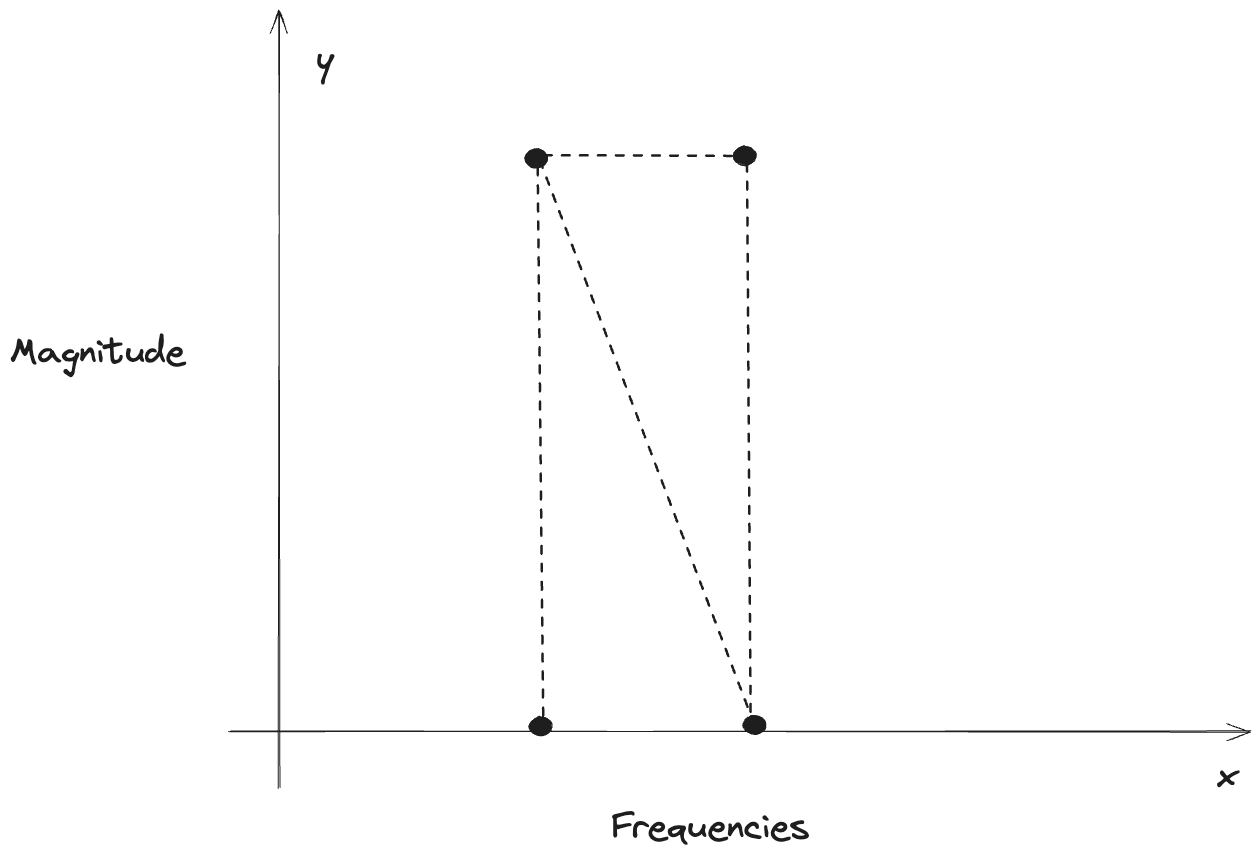
\includegraphics[width=0.5\linewidth]{barchart.png}
    \caption{How points are drawn in bar chart visualization}
    \label{fig:bar}
\end{figure}

If there are more than 3 points then draw a Pygame polygon.

\newpage

\subsubsection{Three frequencies bands visualization}

xf and yf are both normalized in respect to its own maximum and minimum to avoid rendering out of the bound values. The following code accomplishes that:

\begin{lstlisting}
    max_y = max(band_yf) if band_yf else 0
    min_y = min(band_yf) if band_yf else 0
    normalized_data = [(y - min_y) / (max_y - min_y) if max_y > min_y else 0 for y in band_yf]
\end{lstlisting}

This visualization method works by creating 3 centers on the screen based on width and height, splitting xf and yf into 3 arrays, getting the polar coordinates of each magnitude and frequencies in respect to its corresponding centers.

The 3 centers are spaced across the surface evenly using the height and width. Each center represents low, medium, and high bands. xf and yf are also split into 3 even arrays.

\space

\begin{figure}
    \centering
    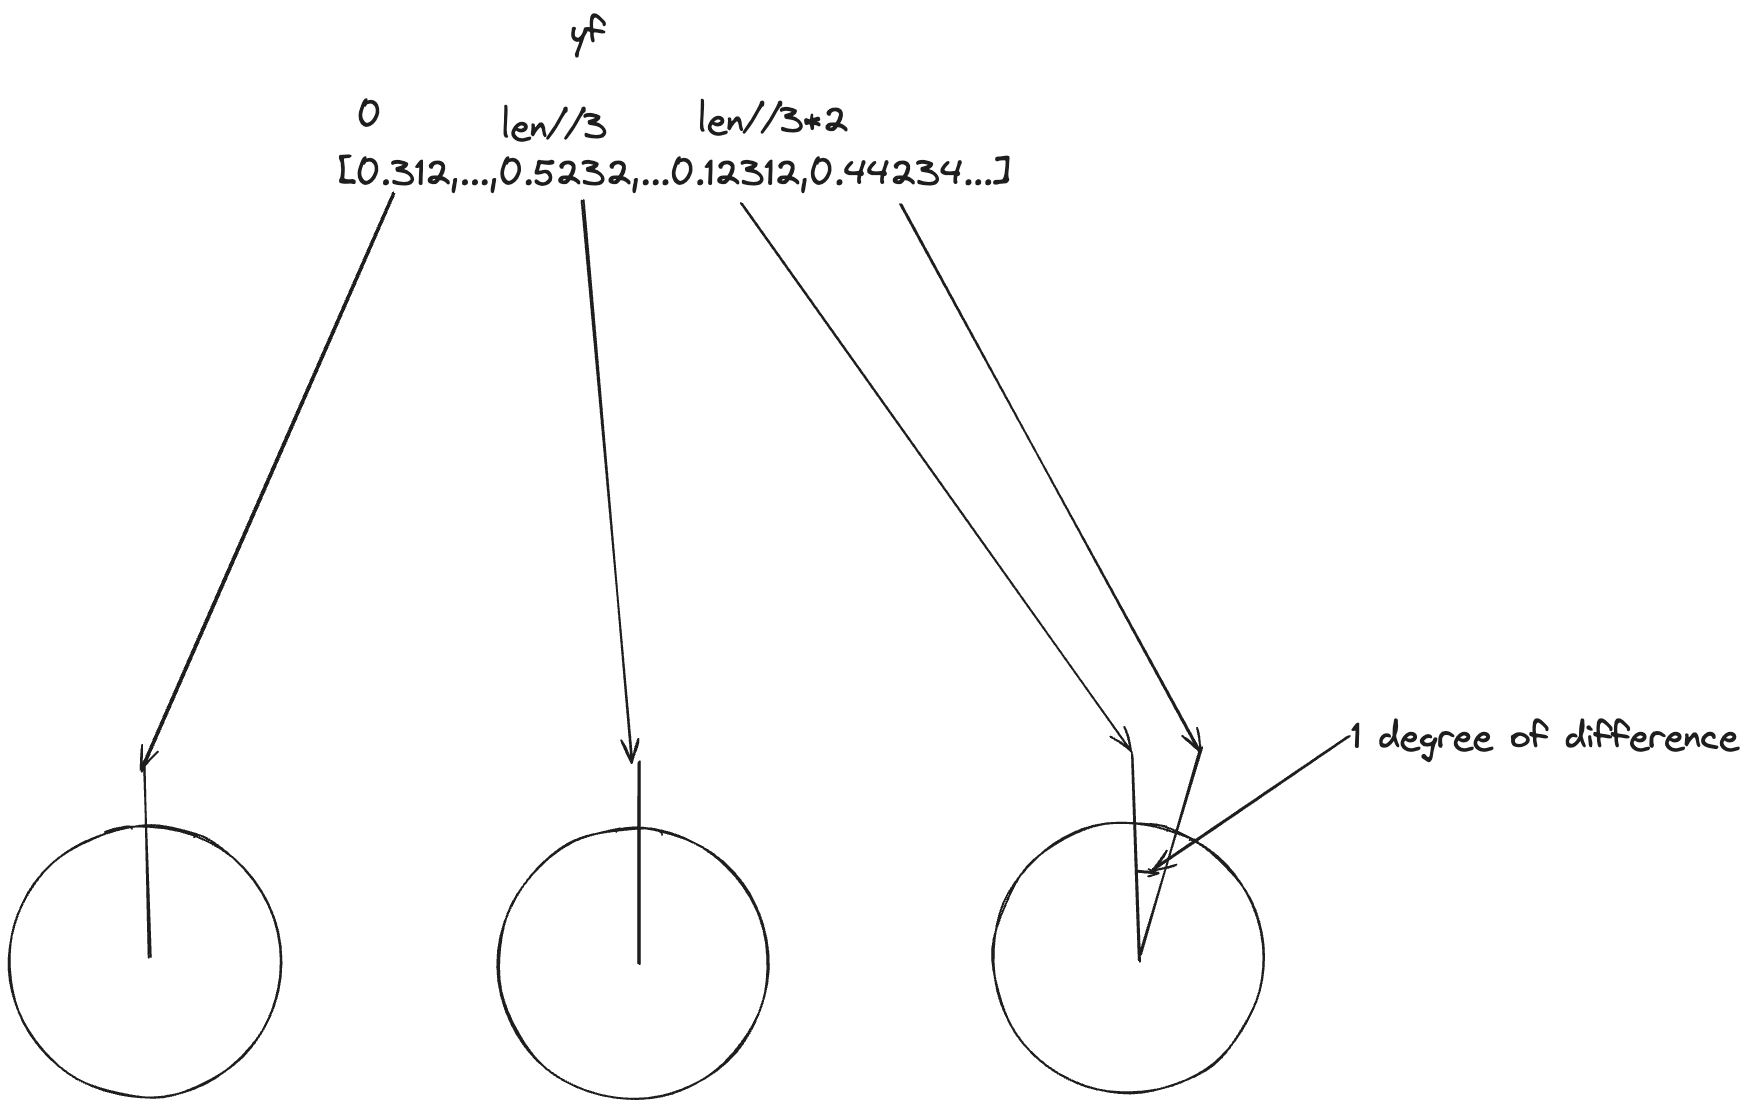
\includegraphics[width=0.5\linewidth]{3circles.png}
    \caption{How points are drawn in three bands visualization}
    \label{fig:circle}
\end{figure}

Using Polar coordinate, the code would calculate the radius and angle based on magnitude and the index of the magnitude. 

For this visualization, sampling is used to get 1080 data points from the input arrays.

\subsubsection{Random color spots visualization}

This visualization technique groups all data points into 50 spots on the surface and display a glow in the background based on the magnitude of each data point within that group.

The 50 spots are randomized on the surface while the glow is applied using a mask on the surface. If the magnitude is higher in each section of the yf array, a circle with lighter color would be drawn in the background and the foreground circle's radius would be extended and blitz to the background, which is how to display overlapping shapes within Pygame. \cite{kinsley}

For this visualization, sampling is used to get 50 points from the input arrays.

\begin{figure}
    \centering
    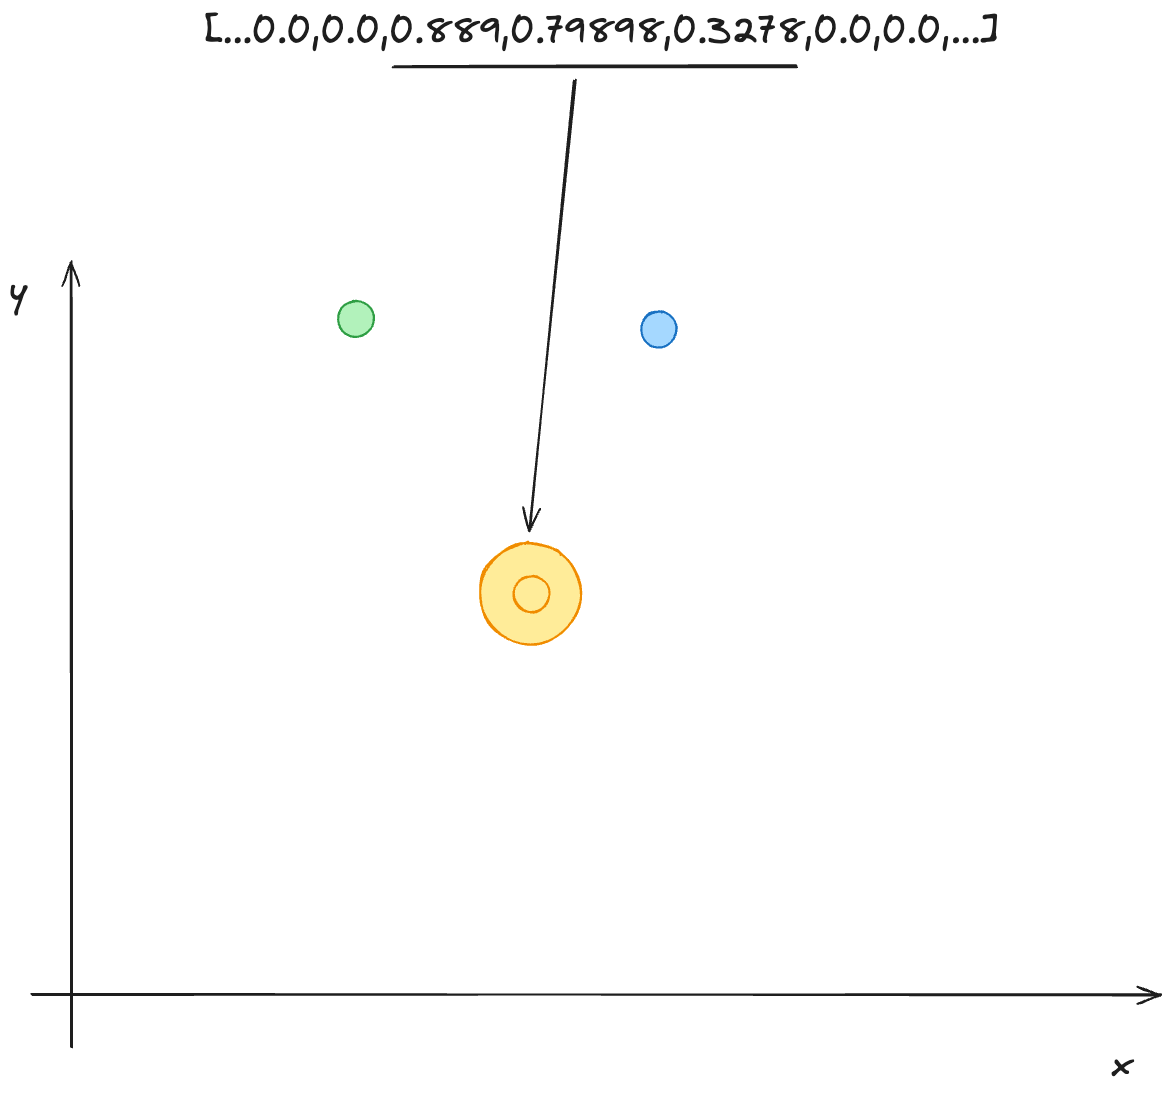
\includegraphics[width=0.5\linewidth]{spots.png}
    \caption{Random spots visualization}
    \label{fig:spots}
\end{figure}



% \section{Typeset Text}\label{sec:typeset_text}

% \subsection{Normal or Body Text}\label{subsec:body}

% Please use a 10pt (point) Times font. Sans-serif or non-proportional fonts can be used only for special purposes, such as distinguishing source code text.

% The first paragraph in each section should not be indented, but all other paragraphs should be.

% \subsection{Title and Authors}

% The title is 14pt Times, bold, caps, upper case, centered. \textbf{Authors' names are omitted when submitting for double-blind reviewing.}

% \subsection{First Page Copyright Notice}

% Please include the copyright notice exactly as it appears here in the lower left-hand corner of the page. It is set in 8pt Times.


% \subsection{Page Numbering, Headers and Footers}

% Do not include headers, footers or page numbers in your submission. These will be added when the publications are assembled.

% \subsection{Line Numbers}

% \textbf{Line numbers should be included in your submitted manuscript,} for reference during reviewing.

% \section{First Level Headings}

% First-level headings are in Times 10pt bold, centered with 1 line of space above the section head, and 1/2 space below it. For a section header immediately followed by a subsection header, the space should be merged.

% \subsection{Second Level Headings}

% Second-level headings are in Times 10pt bold, flush left, with 1 line of space above the section head, and 1/2 space below it. The first letter of each significant word is capitalized.

% \subsubsection{Third and Further Level Headings}

% Third-level headings are in Times 10pt italic, flush left, with 1/2 line of space above the section head, and 1/2 space below it. The first letter of each significant word is capitalized. Using more than three levels of headings is highly discouraged.

% \section{Footnotes and Figures}

% \subsection{Footnotes}

% Indicate footnotes with a number in the text.\footnote{This is a footnote.} Use 8pt type for footnotes. Place the footnotes at the bottom of the page on which they appear. Precede the footnote with a 0.5pt horizontal rule.

% \subsection{Figures, Tables and Captions}

% All artwork must be centered, neat, clean, and legible. All lines should be very dark for purposes of reproduction and art work should not be hand-drawn. The proceedings are not in color, and therefore all figures must make sense in black-and-white form. \textbf{Figure and table numbers and captions always appear below the figure.} Leave 1 line space between the figure or table and the caption. Each figure or table is numbered consecutively. Captions should be Times 10pt. Place tables/figures in text as close to the reference as possible. References to tables and figures should be capitalized, for example, see \figref{fig:example} and \tabref{tab:example}. Figures and tables may extend across both columns to a maximum width of 17.2cm.

% \textbf{To enhance accessibility, we strongly encourage the authors to adopt a color blind friendly color palette when making plots.} For Matplotlib users, the `tableau-colorblind10' and `petroff10' color palettes would be good options, which can be enabled by \texttt{plt.style.use('tableau-colorblind10')} and \texttt{plt.style.use('petroff10')}.

% \begin{table}
%   \centering
%   \begin{tabular}{|l|l|}
%     \hline
%     String value & Numeric value \\
%     \hline
%     Hello ISMIR  & \conferenceyear \\
%     \hline
%   \end{tabular}
%   \caption{Table captions should be placed below the table.}
%   \label{tab:example}
% \end{table}

% \begin{figure}
%   \centering
%   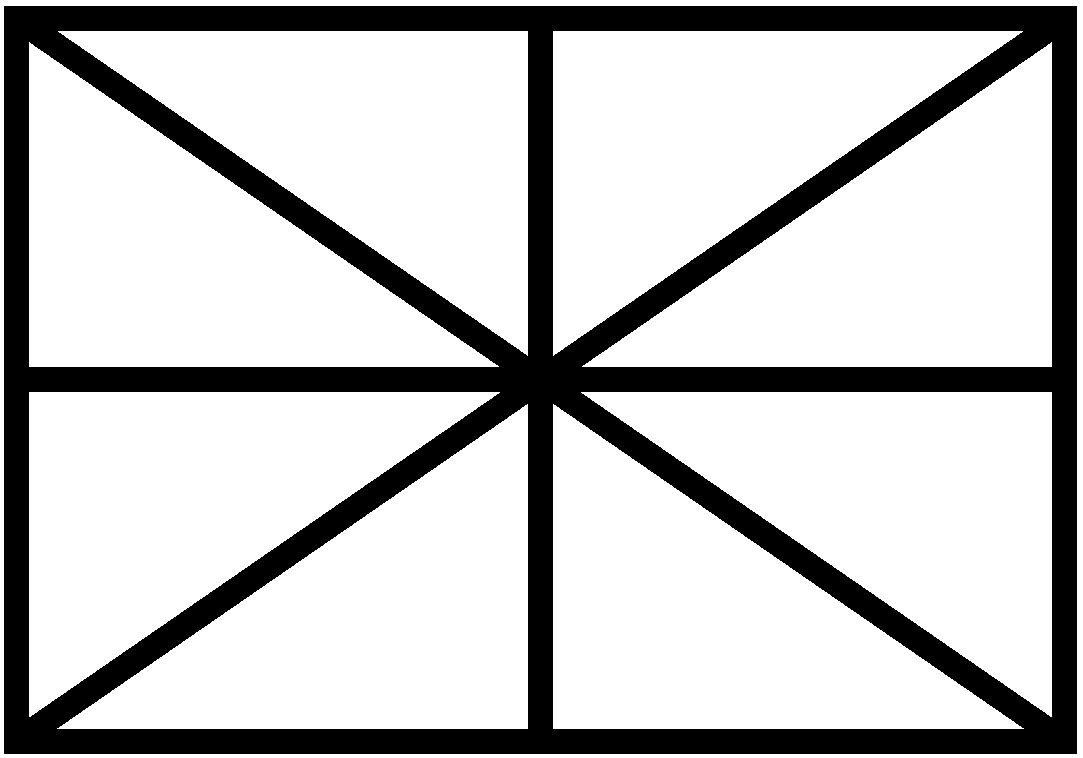
\includegraphics[alt={ISMIR 2025 template example image},width=0.9\linewidth]{example.png}
%   \caption{Figure captions should be placed below the figure.}
%   \label{fig:example}
% \end{figure}

% \section{Equations}

% Equations should be placed on separate lines and numbered. The number should be on the right side, in parentheses, as in \eqnref{relativity}.

% \begin{equation}\label{relativity}
% E=mc^{2}
% \end{equation}

% \section{Citations}

% All bibliographical references should be listed at the end of the submission, in a section named ``REFERENCES,'' numbered and in the order that they first appear in the text. Formatting in the REFERENCES section must conform to the IEEE standard (\url{https://ieeeauthorcenter.ieee.org/wp-content/uploads/IEEE-Reference-Guide.pdf}). Approved IEEE abbreviations (Proceedings $\rightarrow$ Proc.) may be used to shorten reference listings. All references listed should be cited in the text. When referring to documents, place the numbers in square brackets (e.g., \cite{ISMIR17Author:01} for a single reference, or \cite{JNMR10Someone:01,Book20Person:01,Chapter09Person:01} for a range).

% \textbf{As submission is double blind, refer to your own published work in the third person.} That is, use ``In the previous work of \cite{ISMIR17Author:01},'' not ``In our previous work \cite{ISMIR17Author:01}.'' If you cite your other papers that are not widely available (e.g., a journal paper under review), use anonymous author names in the citation, e.g., an author of the form ``A. Anonymous.''

% \section{Acknowledgments}

% You may include an optional Acknowledgments section in your camera-ready version to refer to any individuals or organizations that should be acknowledged in your paper. \textbf{Do not include the Acknowledgments section in your submitted manuscript.} The Acknowledgments section does \textit{not} count towards the page limit for scientific content.

% \section{Ethics Statement}

% You may include an optional Ethics Statement section to provide additional ethical considerations related to your paper. The Ethics Statement section can be included both at submission time and in your camera-ready version. See the Call for Papers for details. The Ethics Statement section does \textit{not} count towards the page limit for scientific content.

% \section{Camera Ready Preparation}\label{sec:cameraready}

% \textbf{The camera-ready version should include the names, affiliations and email addresses of the authors.} Authors' names are centered. The lead author's name is to be listed first (left-most), and the co-authors' names after. If the addresses for all authors are the same, include the address only once, centered. If the authors have different addresses, put the addresses, evenly spaced, under each authors' name. To display the author information in \LaTeX, please remove the global option `submission' when importing the `ismir' package (i.e., \texttt{\textbackslash usepackage\{ismir\}} in line 16).

% \textbf{Please make sure that the author names, paper title and proceedings title are shown correctly in the copyright notice.} For \LaTeX\ users, the proceedings title will be automatically loaded when you remove the global option `submission' when importing the `ismir' package (i.e., \texttt{\textbackslash usepackage\{ismir\}} in line 16). For Word users, you will need to manually replace ``submitted to \textit{ISMIR}, 2025'' to ``in \textit{Proc. of the 26th Int. Society for Music Information Retrieval Conf.}, Daejeon, South Korea, 2025.''

% \textbf{You must also remove all line numbers from the final camera-ready version.} This can be done in \LaTeX\ by removing the global option `submission' when importing the ismir package (i.e., \texttt{\textbackslash usepackage\{ismir\}} in line 16). This can be done in Microsoft Word by selecting ``Layout > Line Numbers > None.''

% % For BibTeX users:
% \bibliography{ISMIRtemplate}

% % For non BibTeX users:
\iffalse
**double check if titles of papers are right format.
i just capitalized first letter of every word but ye
\fi

\newpage
\begin{thebibliography}{citations}

%\bibitem{Author:17}
%E.~Author and B.~Authour, ``The title of the conference paper,'' in {\em Proc.
%of the Int. Society for Music Information Retrieval Conf.}, (Suzhou, China),
%pp.~111--117, 2017.

\bibitem{djfun}
M.~Kaistra, ``Music Visualization GUI,'' GitHub, 2023. [Online]. Available: \url{https://github.com/djfun/audio-visualizer-python/}.

\bibitem{avirzayev}
A.~Rzayev, ``Music Visualization using frequencies,'' GitLab, 2023. [Online]. Available: \url{https://gitlab.com/avirzayev/music-visualizer}.

\bibitem{eklund}
V.-V.~Eklund, ``DBR Dataset,'' Zenodo, Dec. 03, 2017. [Online]. Available: \url{https://doi.org/10.5281/zenodo.1069747}.

\bibitem{picas}
O.~Romani Picas, H.~Parra Rodriguez, D.~Dabiri, and X.~Serra, ``Good-sounds Dataset,'' Zenodo, Jun. 29, 2017. [Online]. Available: \url{https://doi.org/10.5281/zenodo.820937}.

\bibitem{fan}
J.~Fan, M.~Thorogood, and P.~Pasquier, ``Emo-Soundscapes: A Dataset for Soundscape Emotion Recognition,'' in \emph{Proc. Int. Conf. Affective Comput. Intell. Interaction (ACII)}, 2017.

\bibitem{ramires}
A.~Ramiresm, ``Freesound Loop Dataset,'' Zenodo, Jul. 30, 2020. [Online]. Available:\url{https://doi.org/10.5281/zenodo.3967852}

\bibitem{savelsberg}
J.~Savelsberg, ``Visualizing Music Structure Using Spotify Data,''
in {\em ISMIR}, 2021. [Online]. Available: \url{https://archives.ismir.net/ismir2021/latebreaking/000003.pdf}

\bibitem{isaacson}
E.~Isaacson, ``What You See Is What You Get: On Visualizing Music,''
in {\em ISMIR}, 2005. [Online]. Available: \url{https://ismir2005.ismir.net/proceedings/1129.pdf}

\bibitem{takashi}
T.~Takashi, S.~Fukayama, and M.~Goto, ``Instrudive: A music Visualization System Based On Automatically Recognized Instrumentation,''
in {\em ISMIR}, 2018. [Online]. Available: \url{https://archives.ismir.net/ismir2018/paper/000063.pdf}

\bibitem{paulus}
J.~Paulus, M.~M\"uller, and A.~Klapuri, ``Audio-based Music Structure Analysis,''
in {\em ISMIR}, 2010. [Online]. Available: \url{https://ismir2010.ismir.net/proceedings/ismir2010-107.pdf}

\bibitem{thottathil}
I.~A. Thottathil and S.~Thivaharan, ``Virtual Musical Instruments with Python and OpenCV,'' \emph{Journal of Ubiquitous Computing and Communication Technologies}, vol. 5, no. 1, pp. 1–20, Mar. 2023, doi: \url{https://doi.org/10.36548/jucct.2023.1.001}.

\bibitem{mcfee}
B.~McFee, C.~Raffel, D.~Liang, D.~Ellis, M.~McVicar, E.~Battenberg, and O.~Nieto, ``librosa: Audio and Music Signal Analysis in Python,'' in \emph{Proc. Python Sci. Conf.}, 2015, pp. 18–24, doi: \url{https://doi.org/10.25080/majora-7b98e3ed-003}.

\bibitem{suman}
S.~Suman, K. S.~Sahoo, C.~Das, N. Z.~Jhanjhi, and A.~Mitra, ``Visualization of Audio Files Using Librosa,'' in \emph{Proc. 2nd Int. Conf. Math. Model. Comput. Sci.}, ser. Advances in Intelligent Systems and Computing, vol. 1422. Singapore: Springer, 2022, pp. 1–10, doi: \url{https://doi.org/10.1007/978-981-19-0182-9_41}.

\bibitem{kinsley}
H.~Kinsley and W.~McGugan, ``Creating Visuals,'' in \emph{Beginning Python Games Development}. Berkeley, CA: Apress, 2015, pp. 1–20, doi: \url{https://doi.org/10.1007/978-1-4842-0970-7_4}.

\bibitem{ishibashi}
T.~Ishibashi, Y.~Nakao, and Y.~Sugano, ``Investigating Audio Data Visualization for Interactive Sound Recognition,'' in \emph{Proc. 25th Int. Conf. Intell. User Interfaces (IUI '20)}, New York, NY, USA: Association for Computing Machinery, 2020, pp. 67–77, doi: \url{https://doi.org/10.1145/3377325.3377483}.

\bibitem{lagrange}
M.~Lagrange, M.~Rossignol, and G.~Lafay, ``Visualization Of Audio Data Using Stacked Graphs,'' in \emph{ISMIR}, 2018. [Online]. Available: \url{https://zenodo.org/records/1492531}.

\bibitem{knees}
P.~Knees, M.~Schedl, and M.~Goto, ``Intelligent User Interfaces for music Discovery: the past 20 years and what’s to come.'' in \emph{ISMIR}, 2019. [Online]. Available: \url{http://archives.ismir.net/ismir2019/paper/000003.pdf}

\bibitem{Zahid}
S. Zahid, F. Hussain, M. Rashid, M. H. Yousaf, and H. A. Habib, “Optimized Audio Classification and Segmentation Algorithm by Using Ensemble Methods,” Mathematical Problems in Engineering, vol. 2015, pp. 1–11, 2015, Available: \url{https://thesai.org/Publications/ViewPaper?Volume=9&Issue=4&Code=IJACSA&SerialNo=24}

% \bibitem{Person:20}
% O.~Person, {\em Title of the Book}.
% \newblock Montr\'{e}al, Canada: McGill-Queen's University Press, 2021.

% \bibitem{Person:09}
% F.~Person and S.~Person, ``Title of a chapter this book,'' in {\em A Book
% Containing Delightful Chapters} (A.~G. Editor, ed.), pp.~58--102, Tokyo,
% Japan: The Publisher, 2009.

\end{thebibliography}

\end{document}
